\documentclass{article}
\linespread{1.3}
\usepackage[margin=50pt]{geometry}
\usepackage{amsmath, amsthm, amssymb, amsthm, tikz, fancyhdr, graphicx}
\pagestyle{fancy}
\renewcommand{\headrulewidth}{0pt}
\newcommand{\changefont}{\fontsize{15}{15}\selectfont}

\fancypagestyle{firstpageheader}
{
  \fancyhead[R]{\changefont Michael Huang \\ CFRM 420 \\ Homework 5}
}

\begin{document}

\thispagestyle{firstpageheader}

\section*{1.}
{\Large 

% \begin{verbatim}
%   Text enclosed inside \texttt{verbatim}
%   environment 
%   is printed directly 
%   and all \LaTeX{} commands are ignored.
% \end{verbatim}

% \framebox[1.1\width]{\textbf{answer}}

We can calculate the mean and variance of the distribution which we can use to create a normal distribution according to CLT. Since the yearly log return is the sum of 252 iid daily log returns, we can simply find the 95\% confidence interval by taking 252 multiplied by these 95\% confidence interval bands, giving us \framebox[1.1\width]{\textbf{-0.001519248 to 0.001682269}} according to our sample.

}

\section*{2.}
{\Large

\subsection*{(a)}

We plot this in R, and notice that the symmetry of the distribution tends to shift more towards the middle and a more symmetrical distribution rather than asymmetrical as $n$ increases, while the spread generally gets slightly more refined and tighter as $n$ increases.
\begin{figure}[h!]
  \centering
  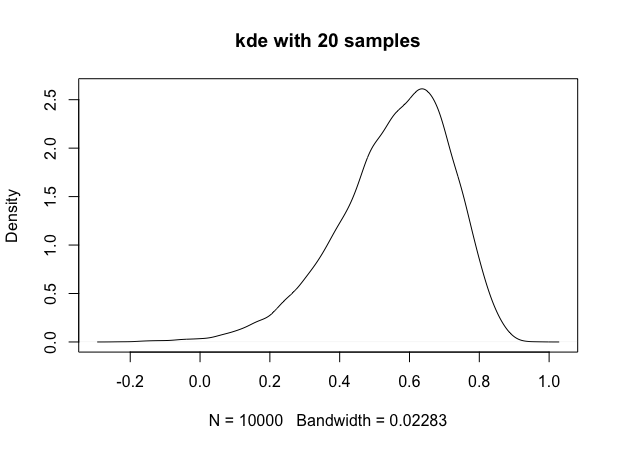
\includegraphics[width=450pt]{hw5_2a_20.png}
\end{figure}
\begin{figure}[t!]
  \centering
  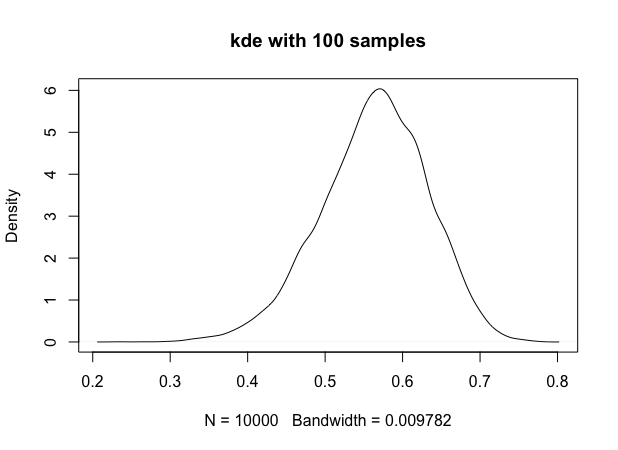
\includegraphics[width=450pt]{hw5_2a_100.png}
\end{figure}
\begin{figure}[t!]
  \centering
  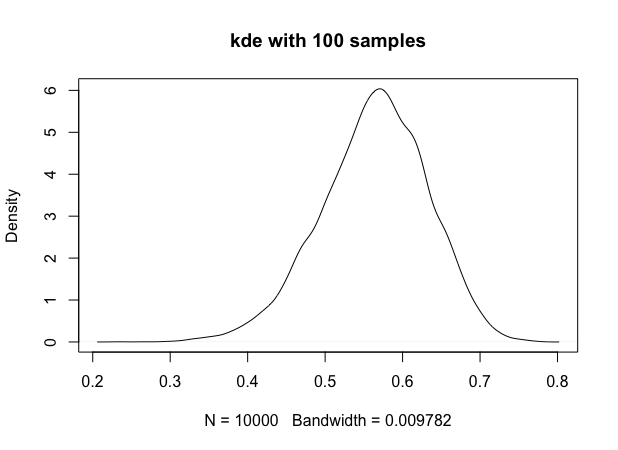
\includegraphics[width=450pt]{hw5_2a_100.png}
\end{figure}
\newpage

\subsection*{(b)}

By definition, we can find each $\text{bias}(\hat{\rho}_n)$ by taking the sum of the means subtracted by the sum of the values: \\
$\text{bias}(\hat{\rho}_{20}) = 
$ -2.00088834390044e-11 \\
$\text{bias}(\hat{\rho}_{100}) = $ 1.45519152283669e-11 \\
$\text{bias}(\hat{\rho}_{500}) = $ 4.54747350886464e-12 \\ \\
By definition, we can find the square root of the variance for each $n$ to estimate $\text{se}(\hat{\rho}_n)$: \\
$\text{se}(\hat{\rho}_{20}) = 0.164072631400487$ \\
$\text{se}(\hat{\rho}_{100}) = 0.0687902431584231$ \\
$\text{se}(\hat{\rho}_{500}) = 0.0306282343447513$

\subsection*{(c)}

As stated, the approximate formulas for large $n$ are $\text{bias}(\hat{\rho}_n) \approx 0$ and $\text{se}(\hat{\rho}_n) \approx \frac{1-\rho^2}{\sqrt{n}} = \frac{1 - (\frac{0.8}{\sqrt{2}})^2}{\sqrt{10000}} = \frac{1 - 0.32}{100} = \frac{0.68}{100} = 0.0068$, since we know that $\rho_{12} = \frac{\sigma_{12}}{\sqrt{\sigma_{11}\sigma_{22}}} = \frac{0.8}{\sqrt{2}}$ and $n = 10000$, as given. \\ \\
Looking at our estimated values, the bias is very close to 0, and only gets better as $n$ increases, while the variance is initially not as close to the actual value but also continues to decrease and get better as $n$ increases.

}

\section*{3.}
{\Large

\subsection*{(a)}

By definition, we know that $\text{bias}(\hat{\theta_1}) = \mathbb{E}[\hat{\theta_1}] - \theta$. We also know that the estimator $\hat{\theta_1}$ is essentially equivalent to doubling the sample mean, or expectation, so we can simplify this expression to be \\
$\text{bias}(\hat{\theta_1}) = \mathbb{E}[\hat{\theta_1}] - \theta = 2 \cdot \mathbb{E}[\theta] - \theta = 2 \cdot \frac{\theta}{2} - \theta = \theta - \theta = 0.$ \\ \\
By definition, we also know that $\text{se}(\hat{\theta_1}) = \sqrt{\text{Variance}(\hat{\theta_1})}$

$\theta / \sqrt{3n}$

\subsection*{(b)}



\subsection*{(c)}

The MSE

$\hat{\theta_2}$

}

\end{document}